\documentclass[aspectratio=169]{../latex_main/tntbeamer}  % you can pass all options of the beamer class, e.g., 'handout' or 'aspectratio=43'
\usepackage{dsfont}
\usepackage{bm}
\usepackage[english]{babel}
\usepackage[T1]{fontenc}
%\usepackage[utf8]{inputenc}
\usepackage{graphicx}
\graphicspath{ {./figures/} }
\usepackage{algorithm}
\usepackage[ruled,vlined,algo2e,linesnumbered]{algorithm2e}
\usepackage{hyperref}
\usepackage{booktabs}
\usepackage{mathtools}

\usepackage{amsmath,amssymb}

\DeclareMathOperator*{\argmax}{arg\,max}
\DeclareMathOperator*{\argmin}{arg\,min}

\usepackage{amsbsy}
\newcommand{\vect}[1]{\bm{#1}}
%\newcommand{\vect}[1]{\boldsymbol{#1}}

\usepackage{pgfplots}
\pgfplotsset{compat=1.16}
\usepackage{tikz}
\usetikzlibrary{trees} 
\usetikzlibrary{shapes.geometric}
\usetikzlibrary{positioning,shapes,shadows,arrows,calc,mindmap}
\usetikzlibrary{positioning,fadings,through}
\usetikzlibrary{decorations.pathreplacing}
\usetikzlibrary{intersections}
\pgfdeclarelayer{background}
\pgfdeclarelayer{foreground}
\pgfsetlayers{background,main,foreground}
\tikzstyle{activity}=[rectangle, draw=black, rounded corners, text centered, text width=8em]
\tikzstyle{data}=[rectangle, draw=black, text centered, text width=8em]
\tikzstyle{myarrow}=[->, thick, draw=black]

% Define the layers to draw the diagram
\pgfdeclarelayer{background}
\pgfdeclarelayer{foreground}
\pgfsetlayers{background,main,foreground}

% Requires XeLaTeX or LuaLaTeX
%\usepackage{unicode-math}

\usepackage{fontspec}
%\setsansfont{Arial}
\setsansfont{RotisSansSerifStd}[ 
Path=../latex_main/fonts/,
Extension = .otf,
UprightFont = *-Regular,  % or *-Light
BoldFont = *-ExtraBold,  % or *-Bold
ItalicFont = *-Italic
]
\setmonofont{Cascadia Mono}[
Scale=0.8
]

% scale factor adapted; mathrm font added (Benjamin Spitschan @TNT, 2021-06-01)
%\setmathfont[Scale=1.05]{Libertinus Math}
%\setmathrm[Scale=1.05]{Libertinus Math}

% other available math fonts are (not exhaustive)
% Latin Modern Math
% XITS Math
% Libertinus Math
% Asana Math
% Fira Math
% TeX Gyre Pagella Math
% TeX Gyre Bonum Math
% TeX Gyre Schola Math
% TeX Gyre Termes Math

% Literature References
\newcommand{\lit}[2]{\href{#2}{\footnotesize\color{black!60}[#1]}}

%%% Beamer Customization
%----------------------------------------------------------------------
% (Don't) Show sections in frame header. Options: 'sections', 'sections light', empty
\setbeamertemplate{headline}{empty}

% Add header logo for normal frames
\setheaderimage{
	% 
\includegraphics[height=\logoheight]{figures/TNT_darkv4.pdf}
	
\includegraphics[height=\logoheight]{../latex_main/figures/luh_logo_rgb_0_80_155.pdf}
	% 
\includegraphics[height=\logoheight]{figures/logo_tntluh.pdf}
}

% Header logo for title page
\settitleheaderimage{
	% 
\includegraphics[height=\logoheight]{figures/TNT_darkv4.pdf}
	
\includegraphics[height=\logoheight]{../latex_main/figures/luh_logo_rgb_0_80_155.pdf}
	% 
\includegraphics[height=\logoheight]{figures/logo_tntluh.pdf}
}

% Title page: tntdefault 
\setbeamertemplate{title page}[tntdefault]  % or luhstyle
% Add optional title image here
%\addtitlepageimagedefault{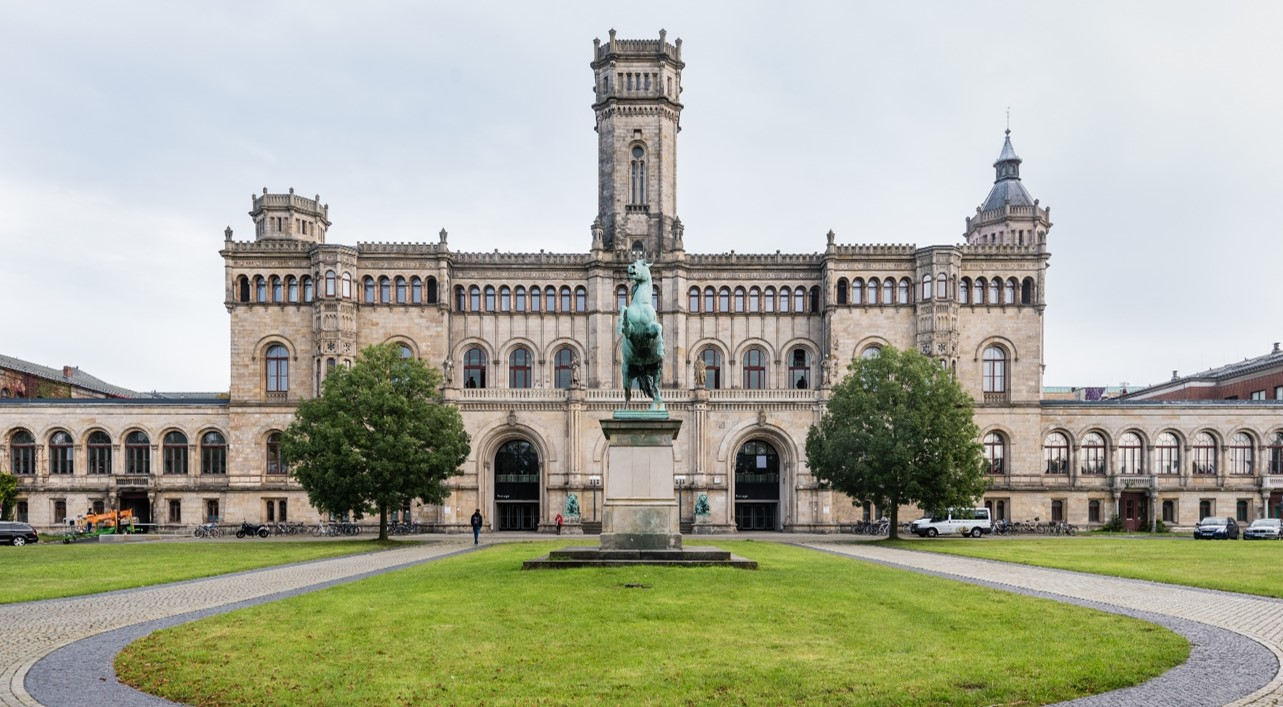
\includegraphics[width=0.65\textwidth]{figures/luh_default_presentation_title_image.jpg}}

% Title page: luhstyle
% \setbeamertemplate{title page}[luhstyle]
% % Add optional title image here
% \addtitlepageimage{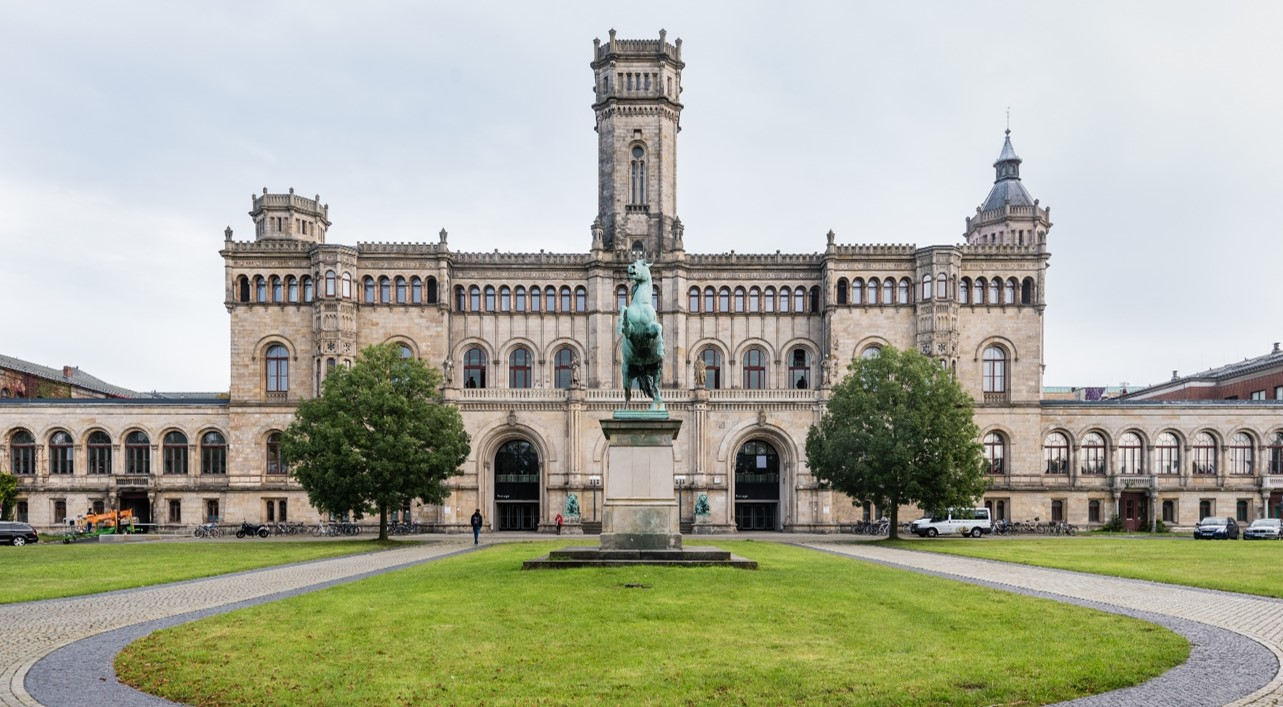
\includegraphics[width=0.75\textwidth]{figures/luh_default_presentation_title_image.jpg}}

\author[Abedjan \& Lindauer]{Ziawasch Abedjan \& Marius Lindauer\\[1em]
	
\includegraphics[height=\logoheight]{../latex_main/figures/luh_logo_rgb_0_80_155.pdf}\qquad
	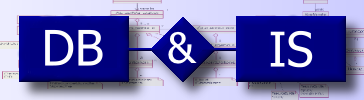
\includegraphics[height=\logoheight]{../latex_main/figures/DBIS_Kurzlogo.png}\qquad

\includegraphics[height=\logoheight]{../latex_main/figures/TNT_darkv4}\qquad

\includegraphics[height=\logoheight]{../latex_main/figures/L3S.jpg}	}
\date{Summer Term 2022; \hspace{0.5em} {
\includegraphics[height=1.5em]{../latex_main/figures/Cc-by-nc-sa_icon.svg.png}}; based on \href{https://ds100.org/fa21/}{[DS100]}
}


%%% Custom Packages
%----------------------------------------------------------------------
% Create dummy content
\usepackage{blindtext}

% Adds a frame with the current page layout. Just call \layout inside of a frame.
\usepackage{layout}


%%% Macros
%\renewcommand{\vec}[1]{\mathbf{#1}}
% \usepackage{bm}
%\let\vecb\bm

\title[Recommender Systems]{DS: Learning}
\subtitle{Recommender Systems}

\graphicspath{ {./figure/} }
%\institute{}


\begin{document}
	
    \maketitle
    
    \begin{frame}{What is the Recommendation Task?}
        \vspace{-1em}
        \begin{itemize}
            \item Only some labels $y_i$ are given
            \begin{itemize}
                \item Classical assumption: no explicit $x_i$ given
                \item But, there could be information about the objects being recommended
            \end{itemize}
            \item Common Example:
            \begin{itemize}
                \item You watched a few movies and rated them from $1-5$ stars
                \item Based on movies rated by others, which movies will you also like?
            \end{itemize}
            \item $\leadsto$ User feedback can be collected in different ways (e.g., watching time, thumbs up, reviews)
            \item \alert{Task}: Extract similarity of different objects $x_i$ based on the labels $y_i$
            \begin{itemize}
                \item Each label consists of an entire (sparse) vector ratings
            \end{itemize}
        \end{itemize}

    \end{frame}

   \begin{frame}{Recommender Approaches}

        \begin{description}
            \item[Collaborative filtering] works by analyzing the behavior and preferences of users, and then recommending items that are preferred by similar users. 
            \begin{description}
                \item[user-based] the system finds users who are similar to the current user and recommends items that these similar users have liked
                \item[item-based] the system finds items that are similar to the items the current user has liked and recommends those similar items.
            \end{description}
           \pause
           \item[Content-based filtering] works by analyzing the recommended items' characteristics and matching them to the user's preferences. The system recommends items with similar features to items that the user has liked in the past
            \item[Matrix factorization] learns the latent factors or features present in the user-item interaction matrix. This approach can effectively handle sparse data and can also handle new items and users that were not present during training.
        \end{description}
       
   \end{frame}

    \begin{frame}{Matrix Multiplication}

        \vspace{-1em}
        \begin{itemize}
            \item Matrix factorization learns latent features or factors that describe the relationships between users and items.
            \item The user-item interaction matrix is decomposed into two matrices: a user matrix and an item matrix
            \begin{description}
                \item[user matrix] represents each user's preferences across all the latent features
                \item[item matrix] represents each item's attributes across all the latent features
            \end{description}
            \item \alert{Result} The dot product of the user and item matrices approximates the user-item interaction matrix, allowing for the prediction of missing ratings
        \end{itemize}

        $$\mathbf{R} \approx \mathbf{P} \times \mathbf{Q}^T = \hat{\mathbf{R}}$$

        \begin{itemize}
            \item $\mathbf{R}$ represents the user-item interaction matrix.
            \item $\mathbf{P}$ represents the user matrix.
            \item $\mathbf{Q}$ represents the item matrix.
            \item $\hat{\mathbf{R}}$ represents the predicted ratings matrix.
        \end{itemize}
      
   \end{frame}

\end{document}